\section{Equilibrium results}\label{sec:results}

\subsection{Competition creates competition}\label{sec:ccc}

The main result compares three economies that differ only in incumbent strength. Against the weak incumbent the
price carries no information and only a zero-cost challenger prepares; against the strong incumbent the price is
informative and a purchase recruits a high-cost challenger; against the very strong incumbent the price stays
informative, while entry returns to its floor. I write \(F_0\), \(F_1\) and \(F_2\) for the three incumbent
distributions.

\begin{proposition}[Competition creates competition]\label{prop:ccc}
Let the classes satisfy the class ranking~\eqref{eq:classes} and have finite means, let \(F_1\) be a continuous
first-order stochastic strengthening of the continuous incumbent distribution \(F_0\), and let \(F_2\) strengthen
\(F_1\) in the same sense. Fix \(0<\pi,\rho,\lambda<1\), \(0<\beta<1/2\), \(c_H>0\) and \(k>0\). Write
\(\Delta_i=\DT(F_i)\), \(B_i=B_{F_i}\), and \(t_{0,i}\) and \(t_{L,i}\) for the proceeds \(t_0\) and \(t_L\) against
\(F_i\), with \(b=(1-\lambda)\beta\) and \(\kappa(\pi)=\min\{m(\pi),1-M(\pi)\}\). Suppose that
\[
\begin{array}{ll}
\text{(H1), the high-cost window:}& B_0(\pi)<c_H<B_1(M(\pi)),\\
\text{(H2), the trading-cost window:}& \Delta_0<k<\rho\kappa(\pi)\Delta_1,\\
\text{(H3), the exclusion condition:}& B_2(M(\pi))<c_H.
\end{array}
\]
Each economy has a unique equilibrium outcome under all four tie rules.
\begin{enumerate}[label=(\roman*),leftmargin=2em]
\item \emph{The weak incumbent \(F_0\).} Both classes abstain, every posterior equals \(\pi\), entry is \(\rho\), and
all orders share the price \(t_{0,0}+\rho[t_{L,0}-t_{0,0}+\Delta_0\pi]\). High-class ownership is \(\pi\rho W_H(F_0)\).
\item \emph{The strong incumbent \(F_1\).} Class \(H\) buys and class \(L\) sells with probability one. The posteriors
after \((-1,0,1)\) are \((m(\pi),\pi,M(\pi))\), and entry is \((\rho,\rho,1)\). Prices rise strictly in this order.
Class entry and total entry are
\[
e_H=\rho+(1-\rho)(b+\lambda),\qquad e_L=\rho+(1-\rho)b,\qquad
\Ent_1=\rho+(1-\rho)(b+\pi\lambda)>\rho.
\]
High-class ownership rises exactly when \(e_HW_H(F_1)>\rho W_H(F_0)\). Class \(H\)'s takeover share rises exactly
when
\begin{equation}\label{eq:a3-share}
e_HW_H(F_1)W_L(F_0)>e_LW_H(F_0)W_L(F_1).
\end{equation}
If class \(H\) outbids the stronger incumbent, \(W_H(F_1)=1\), it also outbids \(F_0\); high-class ownership
rises from \(\pi\rho\) to \(\pi e_H\), and its takeover share is nondecreasing, strictly exactly when
\(W_L(F_0)>0\). If \(W_L(F_0)=0\), that share is one against both incumbents.
\item \emph{The very strong incumbent \(F_2\).} The orders and posteriors are those of part~(ii), entry is \(\rho\)
after every order, and the three prices differ. High-class ownership is \(\pi\rho W_H(F_2)\).
\end{enumerate}
Against each \(F_i\), with \(\mu_i(x)\) and \(e_i(x)\) the posterior and entry after the order \(x\), prices are
\(P_i(x)=t_{0,i}+e_i(x)[t_{L,i}-t_{0,i}+\Delta_i\mu_i(x)]\), the price belief is \(\mu_i(x)\), high-cost
preparation is \([e_i(x)-\rho]/(1-\rho)\), and bids are truthful.
\end{proposition}

The high-cost window (H1) sets entry through acquisition profit: gross
profit at the prior falls short of the high cost against \(F_0\), so an uninformative price recruits no high-cost
challenger, while gross profit at the top posterior exceeds the high cost against \(F_1\), so a purchase can recruit
one. The trading-cost window (H2) fixes trading before any order profile is known: by the trading bound of
Section~\ref{sec:informed}, every correct order earns at most \(\DT(F_0)-k<0\) against the weak incumbent and at
least \(\rho\kappa(\pi)\DT(F_1)-k>0\) against the strong incumbent, so a correct order cannot cover the trading cost
in the first economy and covers it in the second. The exclusion condition (H3) stops recruitment against \(F_2\), where gross
profit at the top posterior falls short of the high cost (the exclusion bound of Section~\ref{sec:inference}).

The trading-cost window is nonempty exactly when \(\DT(F_0)/\DT(F_1)<\rho\kappa(\pi)\), that is, when competition
widens the target-payoff spread enough between the two incumbent distributions. The condition involves the two
distributions, the classes, \(\rho\), the order slot and \(\pi\), and no unit of money, and a prior away from one
half narrows the window, since \(\kappa(\pi)\) falls when the price already leans toward the favored class.
Section~\ref{sec:benchmark} shows that (H1)--(H3) hold together on an open set of parameters.

The additional entry favors the high class, which places a purchase with probability \(b+\lambda\), while the low
class places one with probability \(b\). High-class ownership multiplies entry in class \(H\) by class \(H\)'s chance
of beating the incumbent, and a stronger incumbent can lower that chance when class \(H\) can lose. The ownership
condition in part~(ii) holds whenever the stronger incumbent leaves the high class a good chance to win,
\((1+\rho)W_H(F_1)\ge2\rho W_H(F_0)>0\), and the high class places a purchase more often than not,
\(b+\lambda>1/2\). When class \(H\) outbids \(F_1\), its chance to win is one against both incumbents, so ownership
rises with entry in class \(H\); the stronger incumbent then takes wins only from the low class, and when a low-class
challenger can beat the weak incumbent, the takeovers that go to the challenger shift toward class \(H\).

Values and costs alone give outbidding when class \(H\) has a decisive advantage on a family of incumbent
distributions: against every distribution in the family at which class \(H\)'s gross profit exceeds \(c_H\), class
\(H\) outbids the incumbent. When \(g_H>g_L\), a price recruits a high-cost challenger only where class \(H\)'s gross
profit exceeds \(c_H\), because gross profit at every posterior below one falls short of \(g_H\). Under a decisive
advantage, (H1) therefore gives \(W_H(F_1)=1\), and the takeover-share statement of part~(ii) applies.

Part~(iii) completes the pattern, in which entry first rises and later falls as the incumbent strengthens. Against
the very strong incumbent even the top posterior fails to justify high-cost preparation, while trading stays
informative, and Section~\ref{sec:coexistence} describes where quiet and informative markets coexist between the
three economies. Appendix~\ref{app:prop2} gives the proof and the three equilibrium tuples. Every comparison behind
the result is strict, so the unique outcome in each economy is the same however ties are broken.

\subsection{The example and the fixed-information control}\label{sec:benchmark}

The numbers and figures of the paper come from an example. In it, the two classes are point masses: \(G_H\) puts
all its mass on \(h=\reg{prim_h}\) and \(G_L\) on \(\ell=\reg{prim_ell}\), so the class and the value coincide. The
incumbent is uniform on \([0,r]\), so an increase in \(r\) strengthens it and the strengths form a path. The prior is
\(\pi=\reg{prim_pi}\), the reserve \(p=\reg{prim_p}\), the zero-cost probability \(\rho=\reg{prim_rho}\), the high
cost \(c_H=\reg{prim_cH}\) and the trading cost \(k=\reg{prim_k}\), and money is measured in units of the low value.
The weak, the strong and the very strong incumbent have the strengths \(r_0=\reg{prim_r0}\), \(r_1=\reg{prim_r1}\)
and \(r_2=\reg{prim_r2}\). Values, the reserve and every strength of the path satisfy
\begin{equation}\label{eq:order}
0<p<\ell<r<h.
\end{equation}

In the example's slot the largest likelihood ratio of an order is \(1+u=\eu\), and the liquidity probability is
\(\beta=\reg{beta_B}\). The presence probability is therefore \(\lambda=u\beta/(1+u\beta)=\reg{lambda_B}\), with
\(b=\reg{b_B}\), and the posterior bounds at the prior are \(M(1/2)=\eu/(1+\eu)=\reg{M_half_B}\) and
\(m(1/2)=\reg{m_half_B}\); Appendix~\ref{app:parameters} lists these values and the arithmetic behind each. With the
example's classes and reserve, (H1)--(H3) are strict inequalities between continuous functions of
\((r_0,r_1,r_2,c_H,k,\rho,\pi,\lambda,\beta)\), so they hold on an open set of these parameters that contains the
example.

\begin{corollary}[Recruitment and ownership in the example]\label{cor:ccc-example-short}
In the example at the prior \(1/2\), (H1)--(H3) hold if and only if \(\reg{u_lo_frac}<u<\reg{u_hi_frac}\), that is,
if and only if the top posterior lies between the preparation thresholds of the strong and the very strong
incumbent, \(\tau(r_1)=\reg{M_lo_frac}<M(1/2)<\reg{M_hi_frac}=\tau(r_2)\). When \(1+u=\eu\), as in the example's
slot, they hold if and only if the prior lies between \(\approx\reg{prior_lo_B}\) and \(\approx\reg{prior_hi_B}\). On
this set class \(H\) outbids every incumbent on the path, entry rises from \(\rho\) at \(r_0\) to
\(\rho+(1-\rho)(b+\pi\lambda)\) at \(r_1\) and returns to \(\rho\) at \(r_2\), and high-class ownership rises from
\(\pi\rho\) to \(\pi[\rho+(1-\rho)(b+\lambda)]\).
\end{corollary}

\begin{table}[tbp]
\centering\small\singlespacing
\caption{Acquisition payoffs in the example.}\label{tab:payoffs}
\begin{tabular}{@{}lccc@{}}
\toprule
 & \(r_0=\reg{prim_r0}\) & \(r_1=\reg{prim_r1}\) & \(r_2=\reg{prim_r2}\)\\
\midrule
Proceeds without entry, \(t_0\) & \reg{p2_base_r0_t0} & \reg{p2_base_r1_t0} & \reg{p2_base_r2_t0}\\
Proceeds with a high-class challenger, \(t_H\) & \reg{p2_base_r0_th} & \reg{p2_base_r1_th} & \reg{p2_base_r2_th}\\
Proceeds with a low-class challenger, \(t_L\) & \reg{p2_base_r0_tl} & \reg{p2_base_r1_tl} & \reg{p2_base_r2_tl}\\
Target-payoff spread, \(\DT\) & \reg{Delta_r0} & \reg{Delta_r1} & \reg{Delta_r2}\\
Gross profit of class \(H\), \(g_H\) & \reg{p2_base_r0_gh} & \reg{p2_base_r1_gh} & \reg{p2_base_r2_gh}\\
Gross profit of class \(L\), \(g_L\) & \reg{p2_base_r0_gl} & \reg{p2_base_r1_gl} & \reg{p2_base_r2_gl}\\
Gross profit at the prior, \(B_r(1/2)\) & \reg{Bprior_r0} & \reg{Bprior_r1_B} & \reg{Bprior_r2}\\
Preparation threshold, \(\tau(r)\) & \reg{tau_r0} & \reg{tau_r1} & \reg{tau_r2}\\
\bottomrule
\end{tabular}
\par\medskip
\begin{minipage}{0.92\linewidth}\footnotesize
\textit{Notes.} Point-mass classes \(h\) and \(\ell\), reserve \(p\), incumbent uniform on \([0,r]\). The entries
follow from equation~\eqref{eq:payoffs}. They do not depend on the slot.
\end{minipage}
\end{table}

Table~\ref{tab:payoffs} reports the acquisition payoffs, and the two forces move in opposite directions from \(r_0\)
to \(r_1\): gross acquisition profit at the prior falls from \(\reg{Bprior_r0}\) to \(\reg{Bprior_r1_B}\), while the
target-payoff spread rises from \(\reg{Delta_r0}\) to \(\reg{Delta_r1}\). In the example's slot, entry rises from
\(\reg{entry_r0}\) at \(r_0\) to \(\reg{entry_r1_B}\) at \(r_1\), and high-class ownership from \(\reg{own_r0}\) to
\(\reg{own_r1_B}\). Class \(H\) outbids every incumbent on the path, because \(h\) exceeds \(r_2\), and the strong
incumbent takes wins only from the low class, so class \(H\)'s takeover share rises from \(\reg{share_H_r0}\) to
\(\reg{share_H_r1_B}\). At \(r_2\) entry returns to \(\reg{entry_r2}\) and the three prices still differ;
Table~\ref{tab:outcomes} lists the three equilibrium tuples. With point-mass classes and a uniform incumbent of any
strength, class \(H\) has a decisive advantage exactly when \(c_H\ge(h^2-p^2)/(2h)\), and the example's high cost
exceeds \((h^2-p^2)/(2h)=\reg{cH_DA_floor_B}\): against every uniform incumbent at which a price recruits a
high-cost challenger, class \(H\) outbids the incumbent.

In the example, integration over \(R\) gives
\begin{equation}\label{eq:payoffs}
\begin{aligned}
t_0&=p\Bigl(1-\frac pr\Bigr),&
t_H&=\frac r2+\frac{p^2}{2r},\\
t_L&=\ell-\frac{\ell^2-p^2}{2r},&
g_H&=h-\frac r2-\frac{p^2}{2r},\\
g_L&=\frac{\ell^2-p^2}{2r},&
\DT(r)&=\frac{(r-\ell)^2}{2r},
\end{aligned}
\end{equation}
with the derivatives
\begin{equation}\label{eq:derivatives}
\DT'(r)=\frac12-\frac{\ell^2}{2r^2}>0,\qquad
g_H'(r)=-\frac12+\frac{p^2}{2r^2}<0,\qquad
g_L'(r)=-\frac{\ell^2-p^2}{2r^2}<0,
\end{equation}
and the preparation threshold
\[
\tau(r)=\frac{2rc_H-(\ell^2-p^2)}{2rh-r^2-\ell^2}.
\]
The right side of the class-gap identity of Section~\ref{sec:profits} is \(h-\ell\) at every \(r\). The spread
approaches zero as \(r\) approaches \(\ell\), since the incumbent then almost never outbids a class-\(L\)
challenger, and Table~\ref{tab:payoffs} reports both numbers at the three strengths.

Appendix~\ref{app:prop2} states Corollary~\ref{prop:region} in full. Below the band a purchase at \(r_1\) does not
recruit a high-cost challenger, and above it a conclusion of Proposition~\ref{prop:ccc} fails at \(r_2\) or at
\(r_1\). Table~\ref{tab:region} gives the recruitment region in decimals, with the example's slot and its distance
to each boundary.

\begin{table}[tbp]
\centering\small\singlespacing
\caption{The recruitment region in the example.}\label{tab:region}
\begin{tabular}{@{}lcccc@{}}
\toprule
Parameter & Region & Example & \multicolumn{2}{c}{Margin to the boundary}\\
\cmidrule(l){4-5}
 & & & lower & upper\\
\midrule
Mass ratio \(u\) & \((\reg{u_lo},\reg{u_hi})\) & \reg{u_B} & \reg{margin_u_lo_B} & \reg{margin_u_hi_B}\\
Top posterior \(M(1/2)\) & \((\reg{M_lo},\reg{M_hi})\) & \reg{M_half_B} & \reg{margin_recruit_post_B} & \reg{margin_return_post_B}\\
Presence \(\lambda\) at \(\beta=\reg{beta_B}\) & \((\reg{lambda_lo_B},\reg{lambda_hi_B})\) & \reg{lambda_B} & \reg{margin_lambda_lo_B} & \reg{margin_lambda_hi_B}\\
Presence \(\lambda\) at the largest \(\beta\) & \((\reg{lambda_lo_third},\reg{lambda_hi_third})\) & & & \\
Prior \(\pi\), all three parts & \((\reg{prior_lo_B},\reg{prior_hi_B})\) & \reg{prim_pi} & \reg{margin_prior_lo_B} & \reg{margin_prior_hi_B}\\
Prior \(\pi\), parts (i) and (ii) & \((\reg{prior_lo_B},\reg{prior_ii_hi})\) & \reg{prim_pi} & \reg{margin_prior_lo_B} & \\
Liquidity probability \(\beta\) & \((0,1/3]\) & \reg{beta_B} & & \reg{margin_beta_B}\\
\bottomrule
\end{tabular}
\par\medskip
\begin{minipage}{0.92\linewidth}\footnotesize
\textit{Notes.} The example's auction and costs, strengths \(r_0,r_1,r_2\). Rows 1 to 4 fix the prior at \(1/2\);
rows 5 and 6 fix \(1+u=\eu\). Rows 1 to 5 give the ranges on which (H1)--(H3) hold, and row 6 gives the range for (H1)--(H2). Row 7 gives the
model's liquidity domain at the example's likelihood-ratio bound. Decimal endpoints are rounded to six places; Corollary~\ref{prop:region} in Appendix~\ref{app:prop2} gives the exact
endpoints.
\end{minipage}
\end{table}

Both ends of the band are preparation thresholds: the lower end \(\tau(r_1)\) is the belief that a purchase needs to
recruit a high-cost challenger against the strong incumbent, and the upper end \(\tau(r_2)\) is the belief at which a
purchase would still recruit one against the very strong incumbent. The threshold rises slowly with strength, and
this sets the width of the band: class \(H\) outbids every incumbent on the path, and its expected payment
\(r/2+p^2/(2r)\) rises by less than one half per unit of strength, a change that is small next to the gap
\(g_H-g_L\) in Table~\ref{tab:payoffs}.

Gross profit at every belief falls strictly with strength above \(\ell\), so the exclusion condition (H3) holds at
every strength in \((r_C,h)\), where the entry ceiling \(r_C\approx\reg{rC_B}\) is the strength at which
\(\tau(r)=M(1/2)\); parts~(i) and~(ii) of Proposition~\ref{prop:ccc} hold without the exclusion condition.
Table~\ref{tab:margins} in Appendix~\ref{app:parameters} records every hypothesis and its positive margin in the
example.

\begin{figure}[tbp]
\centering
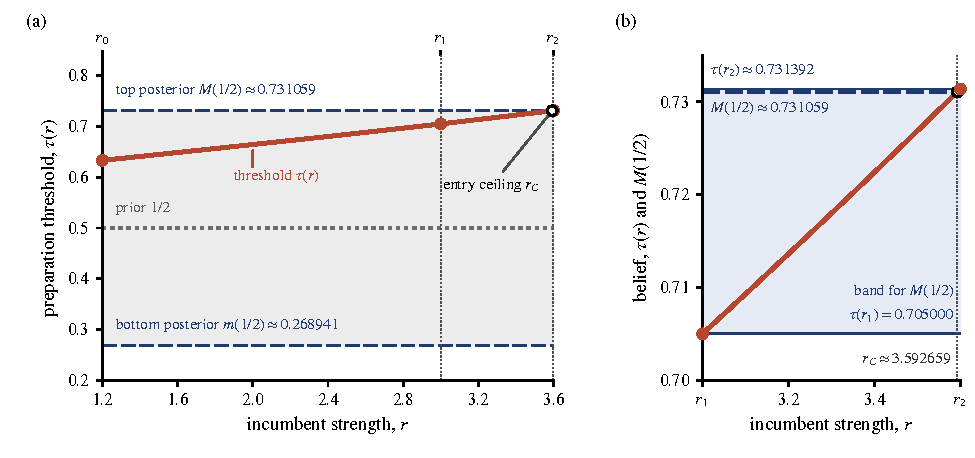
\includegraphics[width=\linewidth]{figures/beliefs.pdf}
\caption{Beliefs and the entry ceiling in the example.}\label{fig:beliefs}
\par\medskip
\begin{minipage}{\linewidth}\footnotesize\singlespacing
\textit{Notes.} Panel (a) plots the preparation threshold \(\tau(r)\) against incumbent strength \(r\). The gray band
covers the posteriors that an investor strategy can produce, from \(m(1/2)\) to \(M(1/2)\). The entry ceiling
\(r_C\) is the strength at which \(\tau(r)\) equals \(M(1/2)\). Panel (b) enlarges the strengths from \(r_1\) to
\(r_2\). Its blue band
holds every top posterior \(M(1/2)\) that puts \(r_C\) between \(r_1\) and \(r_2\); the example's value lies
\(\reg{margin_return_post_B}\) below the upper edge \(\tau(r_2)\).
\end{minipage}
\end{figure}

Figure~\ref{fig:beliefs} shows the preparation threshold along the path: the prior lies below it at every
strength, so an uninformative price never recruits a high-cost challenger, and the threshold rises with strength
until it meets the top posterior at the entry ceiling \(r_C\), just below \(r_2\). Panel~(b) shows the band of
Table~\ref{tab:region} for the top posterior (Corollary~\ref{cor:ccc-example-short}).

Holding the information in the price fixed while the incumbent strengthens removes the reversal. The experiment
fixes the law of the class and of a signal that the challenger observes, the class value laws and the cost law.
Given the class, the signal tells the challenger nothing more about either value. Its own value depends on
the signal only through the class; the incumbent's value is independent of the class and the signal, and the
two values are independent given the class and the signal. The cost is independent of the class, both values and the signal. A stronger incumbent then can only lower entry, for every such experiment and every independent cost law
(Proposition~\ref{prop:control} in Appendix~\ref{app:robustness} gives the formal condition): it lowers gross
profit at every belief, so it can only remove a preparation incentive, and entry falls by exactly the probability
that the cost lies between gross profit against the two incumbent distributions.

In the order slot the experiment fixes \(\lambda\), \(\beta\), \(\pi\), the cost law and both order distributions,
and competitive prices then reveal the same posterior after each order at every strength
(Appendix~\ref{app:beliefs}).

\begin{table}[tbp]
\centering\small\singlespacing
\caption{Equilibrium outcomes and information controls in the example.}\label{tab:outcomes}
\begin{tabular}{@{}lccc@{}}
\toprule
 & \(r_0=\reg{prim_r0}\) & \(r_1=\reg{prim_r1}\) & \(r_2=\reg{prim_r2}\)\\
\midrule
\multicolumn{4}{@{}l}{\emph{Panel A. Equilibrium (Proposition~\ref{prop:ccc})}}\\
Informed orders, classes \(H\) and \(L\) & \((0,0)\) & \((1,-1)\) & \((1,-1)\)\\
Posterior after a sale & \reg{p2_base_r0_mu_minus} & \reg{p2_base_r1_mu_minus} & \reg{p2_base_r2_mu_minus}\\
Posterior after no order & \reg{p2_base_r0_mu_zero} & \reg{p2_base_r1_mu_zero} & \reg{p2_base_r2_mu_zero}\\
Posterior after a purchase & \reg{p2_base_r0_mu_plus} & \reg{p2_base_r1_mu_plus} & \reg{p2_base_r2_mu_plus}\\
High-cost preparation & none & after a purchase & none\\
Price after a sale & \reg{price_r0} & \reg{price_r1_m1_B} & \reg{price_r2_m1_B}\\
Price after no order & \reg{price_r0} & \reg{price_r1_0_B} & \reg{price_r2_0_B}\\
Price after a purchase & \reg{price_r0} & \reg{price_r1_p1_B} & \reg{price_r2_p1_B}\\
Entry \(\Ent\) & \reg{entry_r0} & \reg{entry_r1_B} & \reg{entry_r2}\\
High-class ownership \(\Own_H\) & \reg{own_r0} & \reg{own_r1_B} & \reg{own_r2_B}\\
Expected target proceeds & \reg{p4_base_r0_proceeds} & \reg{p4_base_r1_proceeds} & \reg{p4_base_r2_proceeds}\\
\midrule
\multicolumn{4}{@{}l}{\emph{Panel B. Full orders held fixed (Proposition~\ref{prop:control})}}\\
Entry \(\Ent\) & \reg{p4_frozen_r0_entry} & \reg{p4_frozen_r1_entry} & \\
High-class ownership \(\Own_H\) & \reg{p4_frozen_r0_own} & \reg{p4_frozen_r1_own} & \\
Expected target proceeds & \reg{p4_frozen_r0_proceeds} & \reg{p4_frozen_r1_proceeds} & \\
\midrule
\multicolumn{4}{@{}l}{\emph{Panel C. The challenger does not see the price}}\\
Informed orders, classes \(H\) and \(L\) & \((0,0)\) & \((1,-1)\) & \\
Entry \(\Ent\) & \reg{p4_hidden_r0_entry} & \reg{p4_hidden_r1_entry} & \\
High-class ownership \(\Own_H\) & \reg{p4_hidden_r0_own} & \reg{p4_hidden_r1_own} & \\
Expected target proceeds & \reg{p4_hidden_r0_proceeds} & \reg{p4_hidden_r1_proceeds} & \\
\bottomrule
\end{tabular}
\par\medskip
\begin{minipage}{0.92\linewidth}\footnotesize
\textit{Notes.} The example. Panel A: the unique equilibrium at each strength. Panel B: full orders imposed at
both strengths; at \(r_0\) this profile is a control, not an equilibrium. Panel C: the unique equilibrium when the
challenger decides on its prior. At \(r_2\) the full-order profile is the equilibrium of Panel A.
\end{minipage}
\end{table}

Panel~B of Table~\ref{tab:outcomes} holds full orders fixed at both strengths. Only the top posterior can recruit
a high-cost challenger, because the preparation threshold \(\tau(r)\) exceeds the prior at every strength, so
entry is \(\reg{p4_frozen_r0_entry}\) at every strength up to the entry ceiling \(r_C\approx\reg{rC_B}\) and \(\rho\)
above it. Entry falls by the probability that the cost lies between gross profit at the two strengths, which
is \(\reg{p4_control_crossing_r0_r1}\) from \(r_0\) to \(r_1\) and \(\reg{p4_control_crossing_r1_r2}\) from
\(r_1\) to \(r_2\) (Proposition~\ref{prop:control}): with information fixed, entry stays
constant from \(r_0\) to \(r_1\) and falls above the entry ceiling.

Panel~C hides the price from the challenger, which then decides on its prior and prepares only at zero cost, so
entry stays at \(\reg{p4_hidden_r0_entry}\) at both strengths even though the investor trades fully at \(r_1\). The
two controls together locate the reversal in the information that trading generates: incumbent strength changes
that information, and the entry response to it exceeds the direct deterrence effect of a stronger incumbent at
fixed information.

\subsection{Coexistence}\label{sec:coexistence}

Between the weak and the strong incumbent of Proposition~\ref{prop:ccc}, two equilibria can hold against the same
incumbent. In a quiet market the investor does not trade, the price carries no information, and entry stays at its
floor; in the informative market that coexists with it, a purchase recruits a high-cost challenger. The two numbers
of Section~\ref{sec:twonumbers} decide where both exist: the threshold must lie above the prior and within reach of
a purchase, and the spread must be wide enough that a purchase that just reaches the threshold covers the trading
cost, yet narrow enough that no order against an uninformative price earns more than it.

\begin{proposition}[Quiet and informative markets]\label{prop:coexistence}
Let the classes satisfy the class ranking~\eqref{eq:classes}, let \(0<\pi<1\), \(0<\rho<1\), \(k>0\) and a slot
\((\lambda,\beta)\) be given, and let an indifferent investor mix over its best orders and an indifferent high-cost
challenger prepare. Take an incumbent distribution with a positive spread \(\DT\) and \(g_H>g_L\), and write \(\tau\)
for its preparation threshold.
\begin{enumerate}[label=(\alph*),leftmargin=2em]
\item A quiet market and an informative market coexist if and only if
\[
\pi<\tau\le M(\pi),\qquad \frac{k}{1-\tau}\le\DT\le\frac{k}{\rho\max\{\pi,1-\pi\}}.
\]
The informative market is then unique: class \(L\) abstains, only a purchase recruits a high-cost challenger, and
entry is
\[
\rho+(1-\rho)\min\Bigl\{\frac{(1-\pi)\,b\,\DT}{k},\;b+\pi\lambda\Bigr\},
\]
which rises strictly with the spread while class \(H\) mixes between a purchase and abstention and is constant once
class \(H\) buys for sure.
\item Along a path of such distributions, the strengths at which a quiet market coexists with an informative market
in which class \(H\) buys for sure form an interval, and every other strength with coexistence lies below it. Every
gap in coexistence lies at spreads too narrow for a sure purchase to pay.
\item Along a path on which the product of the spread and \(g_H-c_H\) does not fall with strength, the strengths
with coexistence form an interval, at every prior. Uniform incumbents on \([0,r]\), with \(r\) in a closed interval
above the reserve, satisfy this condition when every low-class value lies between the reserve and the lowest
strength, every high-class value is at least the highest strength, and class \(H\)'s mean value exceeds the highest
strength by at least \(c_H\).
\end{enumerate}
\end{proposition}

Coexistence comes from the entry response itself. In a quiet market entry stays at its floor after every order, so an
informed order earns at most \(\rho\max\{\pi,1-\pi\}\) times the spread, and the upper bound on the spread keeps that
from exceeding the trading cost. An informative market changes the entry response to a purchase, and with it the
return to trade: a purchase that reaches the threshold recruits, and the lower bound on the spread lets it cover the
trading cost.

Entry rises with the spread while class \(H\) mixes, because the purchase rate adjusts. While class \(H\) mixes, a
recruiting purchase earns exactly the trading cost, so a wider spread needs a more informative purchase; the purchase
rate rises, and entry rises with it until class \(H\) buys for sure. Entry depends on the incumbent only through the
spread, so between two incumbents at which the markets coexist, entry in the informative market is at least as high
against the one with the wider spread.

A stronger incumbent never narrows the spread, and where the threshold is positive it never lowers the threshold, so
the two numbers pull in opposite directions: a wider spread raises what a recruiting purchase earns, and a higher
threshold makes recruitment harder. As the incumbent strengthens, the economy can enter the region, leave it, and
enter it again. The strengths with a sure purchase are never split, because each condition that defines them holds on
one side of a single strength, and a mixed purchase needs a narrower spread than a sure one, so the other strengths
with coexistence lie below them. When class \(H\)'s gross profit exceeds the high cost against the weakest incumbent,
the whole set stays in one piece if the spread grows, in proportion, at least as fast as that excess shrinks;
part~(c) states the condition as a product, which does not fall.

The example satisfies the condition of Proposition~\ref{prop:coexistence}(c): its incumbent is uniform, \(\ell\) lies
between \(p\) and \(r_0\), and \(h\) exceeds \(r_2\) by more than \(c_H\), so at every prior the strengths with
coexistence form one interval. At the prior \(1/2\) the interval starts at \(r_A\), where a purchase that just
reaches the threshold and recruits earns the trading cost, and it ends at \(r_N\), where a unit order against an
uninformative price earns the trading cost. Class \(H\) buys for sure from \(r_F\), where a full purchase that
recruits earns the trading cost.

\begin{corollary}[Coexistence in the example]\label{cor:example-coexistence-short}
In the example at the prior \(1/2\), let the slot lie in the band of Corollary~\ref{cor:ccc-example-short}, and let an
indifferent investor mix over its best orders and an indifferent high-cost challenger prepare. An equilibrium exists
at every strength of the path from \(r_0\) to \(r_2\), and the strengths at which a quiet market and an informative
market coexist form the interval \([r_A,r_N]\). In the informative market that coexists with a quiet market, entry
is \(\rho+(1-\rho)\min\{b\DT(r)/(2k),\,b+\lambda/2\}\); it rises strictly on \([r_A,r_F]\) and is constant on
\([r_F,r_N]\). With a full purchase, entry keeps this value up to the entry ceiling \(r_C\) and equals \(\rho\) above
it.
\end{corollary}

\begin{figure}[tbp]
\centering
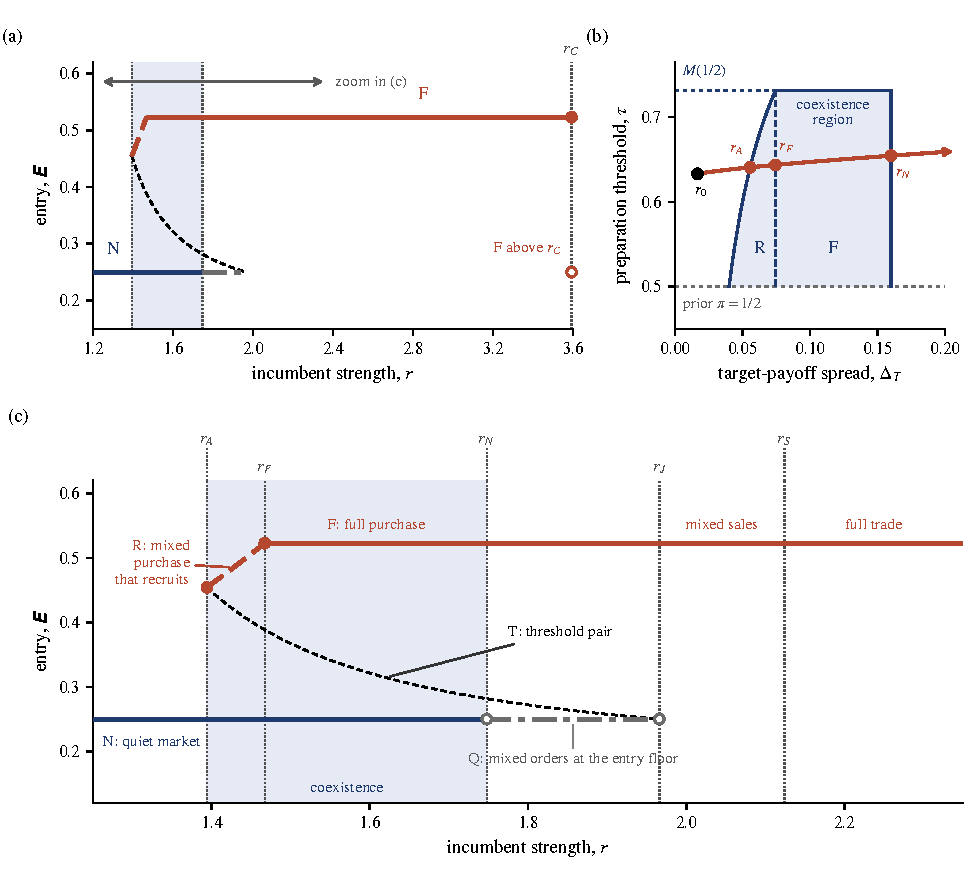
\includegraphics[width=\linewidth]{figures/coexistence.pdf}
\caption{Entry and the coexistence region along the example's path.}\label{fig:coexistence}
\par\medskip
\begin{minipage}{\linewidth}\footnotesize\singlespacing
\textit{Notes.} The example at the prior \(1/2\), when an indifferent investor may mix over its best orders and an
indifferent high-cost challenger prepares. Panels (a) and (c) show entry against incumbent strength \(r\) in each
equilibrium of Corollary~\ref{cor:example-coexistence}. Panel (a) covers the path from \(r_0\) to \(r_2\), and panel
(c) enlarges the strengths around the coexistence interval, which the blue band marks from \(r_A\) to \(r_N\). The
figure labels a quiet market by N, a mixed purchase that recruits by R, a full purchase by F, mixed orders at the
entry floor by Q and the threshold pair by T. The thin dashed line is the threshold pair~T. At \(r_A\) its purchase
recruits with probability one, and it is an equilibrium under the default tie rules; on \((r_A,r_J]\) it is an
equilibrium when an indifferent high-cost challenger may prepare with any probability. With a full purchase the low
class abstains up to \(r_N\), mixes from \(r_N\) to \(r_S\), and sells with probability one from \(r_S\); above the
entry ceiling \(r_C\), entry with a full purchase equals \(\rho\). Panel (b) draws the region of
Proposition~\ref{prop:coexistence}(a) at the example's slot, in the plane of the target-payoff spread \(\DT\) and
the preparation threshold \(\tau\): \(1/2<\tau\le M(1/2)\) and \(k/(1-\tau)\le\DT\le2k/\rho\). The dotted lower
edge, where \(\tau\) equals the prior, lies outside the region, and the other three edges belong to it. The dashed line
\(\DT=k/(1-M(1/2))\) divides the mixed purchase R, on its left, from the full purchase F. The curve traces
\((\DT(r),\tau(r))\) from \(r_0\): it enters the region at \(r_A\), reaches full purchases at \(r_F\), leaves the
region at \(r_N\), and continues towards \(r_1\) and \(r_2\) beyond the panel. Filled markers belong to a curve, and
open markers do not.
\end{minipage}
\end{figure}

In the example's slot, coexistence runs from \(r_A\approx\reg{rA}\) to \(r_N\approx\reg{rN}\), and class \(H\) buys
for sure from \(r_F\approx\reg{rF_B}\). Between \(r_A\) and \(r_F\) class \(H\) buys at the rate
\(b\,[\DT(r)/k-2]\), which rises with the spread until it reaches \(\lambda\) at \(r_F\), so entry in the informative
market is \(\reg{entry_rA_B}\) at \(r_A\), \(\reg{entry_mb_r140_B}\) at \(\reg{str_r140}\) and
\(\reg{entry_mb_r145_B}\) at \(\reg{str_r145}\); from \(r_F\) it stays at \(\reg{entry_r1_B}\) up to the entry
ceiling \(r_C\approx\reg{rC_B}\). Above \(r_N\) the informative market with a full purchase remains, and on
\((r_N,r_J)\), with \(r_J\approx\reg{rJ}\), mixed orders at the entry floor join it. The low class abstains up to
\(r_N\), mixes on \((r_N,r_S)\) and sells for sure from \(r_S\approx\reg{rS_B}\), the strength at which a full sale
earns the trading cost. Figure~\ref{fig:coexistence} draws the path through the region and the entry it produces,
and Appendix~\ref{app:coexistence} lists every equilibrium along the path.

The example's high cost lies between the two bounds that these conditions place on it. It is at most
\(h-r_2=\reg{cH_afford_ceiling_B}\), so class \(H\)'s value covers the high cost against the strongest incumbent
and Proposition~\ref{prop:coexistence}(c) applies, and it is at least \((h^2-p^2)/(2h)=\reg{cH_DA_floor_B}\), so
class \(H\) has the decisive advantage of Section~\ref{sec:ccc}.

Coexistence also holds away from the even prior. In the example's slot it starts at the same strength \(r_A\) for
every prior between \(\approx\reg{piA_lo_B}\) and \(\approx\reg{piA_hi}\), and it starts later, where the prior
reaches the threshold, for priors up to \(\approx\reg{pimax}\). Below \(\approx\reg{piA_lo_B}\) even the top
posterior cannot reach the threshold once a purchase can pay for itself, and from \(\approx\reg{pimax}\) on, the
quiet market ends before the prior falls below the threshold. Appendix~\ref{app:coexistence} gives the coexistence
set at every prior (Corollary~\ref{prop:priors}).
